%&latex
\documentclass[12pt]{article}
\usepackage{amsmath}
\usepackage{graphicx,psfrag,epsf}
\usepackage{enumerate}
\usepackage{natbib}
\usepackage{url} % not crucial - just used below for the URL 

%\pdfminorversion=4
% NOTE: To produce blinded version, replace "0" with "1" below.
\newcommand{\blind}{0}

% DON'T change margins - should be 1 inch all around.
\addtolength{\oddsidemargin}{-.5in}%
\addtolength{\evensidemargin}{-.5in}%
\addtolength{\textwidth}{1in}%
\addtolength{\textheight}{1.3in}%
\addtolength{\topmargin}{-.8in}%

\font\tt=rm-lmtl10
\font\itt=rm-lmtlo10
\font\btt=rm-lmtk10
\font\bitt=rm-lmtko10



\begin{document}

%\bibliographystyle{natbib}

\def\spacingset#1{\renewcommand{\baselinestretch}%
{#1}\small\normalsize} \spacingset{1}


%%%%%%%%%%%%%%%%%%%%%%%%%%%%%%%%%%%%%%%%%%%%%%%%%%%%%%%%%%%%%%%%%%%%%%%%%%%%%%

\if0\blind
{
  \title{\bf The Hedging Hyperprior. A simple and easy to teach reformulation of the Modified Power Prior}
  \author{Stephen D. Simon 1\thanks{
    This work was partially supported by an NIH grant from NCI awarded to The University of Kansas Cancer Center (The KUCC) \#1 P30 CA168524.}\hspace{.2cm}\\
    Department of Biomedical and Health Informatics,\\University of Missouri-Kansas City\\
    Yu Jiang\\
    Division of Epidemiology, Biostatistics, and Environmental Health,\\University of Memphis\\
    and \\
    Byron J. Gajewski\\
    Department of Biostatistics \& Data Science,\\University of Kansas Medical Center}
  \maketitle
} \fi

\if1\blind
{
  \bigskip
  \bigskip
  \bigskip
  \begin{center}
    {\LARGE\bf Title}
\end{center}
  \medskip
} \fi

\bigskip
\begin{abstract}
In many settings, Bayesian models rely on flat or non-informative prior distributions, but sometimes you might prefer to use an informative prior distribution. An informative prior will provide you with added precision, but if your data are inconsistent with the prior distribution, you may wish that you had used a flat prior instead. The Modified Power Prior is commonly used to reweight an informative prior downward when the data is inconsistent with the prior, but the mathematical details are difficult, especially for students new to Bayesian models. In addition, this approach does not provide any guidance on how to fit this model using standard Bayesian analysis programs. In this paper, we present the hedging hyperprior, a simple modification of the informative prior through the use of a single hyperparameter. We show how this works for the beta-binomial model and demonstrate its equivalence in this setting to the Modified Power Prior. We illustrate the joint prior distribution of the binomial proportion and the hedging hyperprior with a three dimensional surface which offers an intuitive demonstration of how and why this hyperparameter works to downweight the informative prior. We present the hedge trace, a simple two dimensional plot that shows exactly where the hyperprior downweights the informative prior and by how much. This allows students to directly compare different distributions for the hyperparameter. The hedging hyperprior provides a simple and easy to teach framework for using informative priors safely.


\end{abstract}

\noindent%
{\it Keywords:}  Beta-binomial model, Informative prior, hyperprior
\vfill

\newpage
\spacingset{1.45} % DON'T change the spacing!
\section{Introduction}
\label{sec:intro}

Stephen Senn is a delightful source for quotes that are humorous but which slyly illustrate important statistical principles. One of these quotes, found in (\cite{senn08}, page 46.) is especially relevant to Bayesian data analysts. "A Bayesian is one who, vaguely expecting a horse and catching a glimpse of a donkey, strongly concludes he has seen a mule." 

The horse is the prior distribution, and donkey is the data, and a Bayesian will combine these, even when they are so different to produce something that is neither horse nor donkey. You avoid this problem, of course, if you use a flat or non-informative prior as it puts all (or almost all) of the weight on the data. There are situations, however, where you can and should use an informative prior.

In previous research involving patient accrual models (\cite{gajewski08}), we developed a Bayesian predictive model that asked the researchers for their opinion about how long a proposed clinical trial would take and then asked how confident they were about this estimate on a scale of 1 to 10. Their level of confidence would provide a preliminary estimate of the precision of the prior distribution. An answer of 5, for example, would produce a suggested prior distribution with a precision comparable to 50\% of the planned sample size. An answer of 2 would provide a much more variable prior distribution with a precision comparable to 20\% of the proposed sample size.

We did not, however, allow a value of 0, corresponding to a flat or non-informative prior. In the setting of patient accrual, a flat prior would be nonsensical. It would be like saying, "I'm not sure, maybe the trial will take 10 days and maybe it will take 10 years. Either value would be quite reasonable." A researcher who could not narrow down the time frame any more than this would be unqualified to conduct the research.

In the context of patient accrual, an informative prior has the additional advantage in that it allows you to predict the duration of the trial before any data are collected and stabilizes the estimated predicted duration of the trial when only a small amount of accrual data are available.

A second example where informative priors make sense is when you have information about the placebo response rate that you'd expect to see in your current trial based on the placebo response rate that you observed in previous trials. Every drug trial is different because every new drug is different, but the placebo arm is often run under the exact same conditions in each trial. You can incorporate the information of these placebo patients using a Bayesian meta-analytic approach. You could use this approach even for drugs that are substantially different because you allow the treatment response rate to have a vague or uninformative prior. A useful example of this approach appears in \cite{walley15}.

You could even argue in this setting that use of a flat prior is unethical. You are ignoring valuable information from the previous placebo groups, information that could minimize patient risk by reducing the sample size of the current trial and reducing the number of patients who receive the placebo.

While informative prior distributions can be very useful, they can lead to serious problems if the data are substantially inconsistent with the prior distribution. Several solutions have been proposed, including the Modified Power Prior (\cite{ibrahim03}), but these approaches are difficult to explain, especially to students just learning about Bayesian inference.

We propose a simple modification of the Bayesian model, the hedging hyperprior, that adds a single hyperparameter to allow downweighting of the informative prior when there is a large discrepancy between the prior distribution and the data. The modification is simple to explain, and offers an intuitive visual presentation of how this hyperparameter protects against a strongly discrepant informative prior. You can easily fit this Bayesian model using standard software like BUGS, JAGS, or Stan.

In section \ref{sec:bb} of this article, we show a simple case of the beta-binomial problem with an informative prior, both when the data are reasonably consistent with the prior distribution and when they are markedly different. In section \ref{sec:hh}, we show how adding a hyperprior on the precision of the prior distribution can sharply downweight the strength of the prior distribution when the data are inconsistent with the prior distribution. In section \ref{sec:equiv}, we summarize the Modified Power Prior and illustrate that the hedging hyperprior in the beta-binomial setting is equivalent to the Modified Power Prior. In section \ref{sec:pr}, we compare several choices for the distribution of the hyperparameter.

\section{A beta-binomial model with an informative prior distribution}
\label{sec:bb}
Consider a Bayesian model for a binomial distribution with a beta prior. 

\begin{figure}
\begin{center}
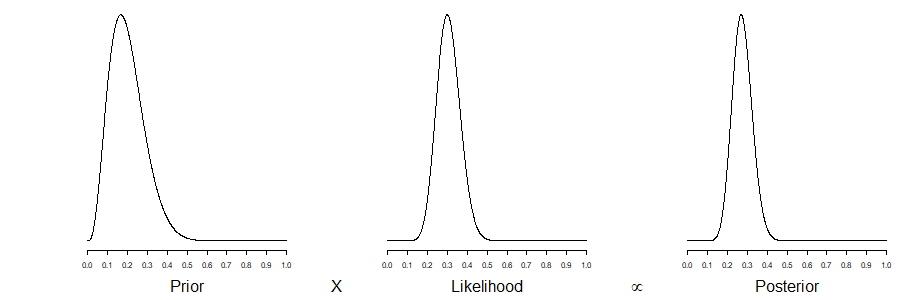
\includegraphics[width=6in]{fig1.png}
\end{center}
\caption{Prior, likelihood, and posterior for a nice beta-binomial model \label{fig:fig_nice}}
\end{figure}

Let's start with a prior distribution which is beta(4, 16). This informative prior, shown in Figure \ref{fig:fig_nice}, has a mean of 0.2 and places most of the weight on values for the binomial proportion between 0.1 and 0.4. The precision of the beta distribution is equal to the sum of the two parameters, alpha and beta, which is 20 in this case. This is commonly called the prior sample size. A prior sample size of 20 implies that if you collected 20 observations, the Bayesian model would give equal weight to those 20 observations and the prior distribution.

Suppose that you collect data from a clinical trial and find that among 60 subjects, 18 were classified as successes and 42 as failures or a proportion of successes equal to 0.3. That's just a bit higher than your prior mean, but still a fairly reassuring result.

The likelihood for this data, also shown in Figure \ref{fig:fig_nice}, reaches a maximum at 0.3 but the likelihood for values between 0.2 and 0.4 are also reasonable. You combine the prior and the likelihood to get a posterior distribution that is beta(4+18=22, 42+18=58). One of the key benefits of the Bayesian model is the extra precision that the prior distribution provides. The posterior sample size in this example is 80, which is the sum of the prior sample size (20) and the size of the data itself (60).

The posterior distribution, beta(22, 58), has mean of 0.275 and a 95\% credible interval of 0.18 to 0.38. The posterior mean is between the mean of the prior distribution and the mean of the data and closer to the mean of the data because the sample size of your data is larger than the sample size of your prior distribution.

You don't really need statistical software to solve this problem, but to set the stage for later Bayesian models, let's see how you would use R (\cite{r17}) and JAGS (\cite{plummer16}) to solve this simple beta-binomial model. The code shown here is easily adapted to BUGS (\cite{lunn00}) or STAN (\cite{carpenter17}). Table \ref{tab:bb_code} shows four lines of JAGS code that you store in a simple text file. Name it jbb.txt and store it in the current working directory of your R session. Then run the R code that is also shown in Table \ref{tab:bb_code}.

\linespread{1}

\begin{table}
\caption{The classic beta-binomial model. \label{tab:bb_code}}

Beta-binomial formulation \\

$\pi \sim beta(\alpha, \beta)$ \\
$x \sim Binomial(n, \pi)$ \\

JAGS code for the beta-binomial model (store in jbb.txt). 

\begin{verbatim}
model {
  pi ~ dbeta(a,b)
  x ~ dbin(pi,n)
}
\end{verbatim}

R code

\begin{verbatim}
library("rjags")
dat.bb <- list(a=4,b=16,x=18,n=60)
mod.bb <- jags.model("jbb.txt",dat.bb)
update(mod.bb,1000)
out.bb <- coda.samples(mod.bb, "pi", 1000)
\end{verbatim}
\end{table}

\linespread{1.6}

You are probably quite happy with yourself at this point. You have a posterior mean which is close to what the data tells you. You don't mind that the mean is a bit smaller because you had some information, possibly from historical data, possibly from interviews with experts in the area, and possibly straight from your gut, that told you that the proportion might be a bit smaller. What really makes you happy, though, is that you have some extra precision because you were smart enough to use an informative prior distribution. Thank you, Reverend Bayes.

Now imagine yourself in a setting that is not quite as nice. A setting that is quite bad. More than bad, actually, disastrously bad. Prepare yourself because the next few paragraphs are going to be rather upsetting.  

Let's suppose the you have the same prior distribution, beta(4,16), but now your data have 54 successes and only 6 failures. The data are telling you that the binomial proportion is probably around 0.9, but your prior distribution is concentrated around 0.2. When you combine the prior horse with the data donkey, you get a distinctly mulish beta(58, 22) with a posterior mean of 0.725 (Figure \ref{fig:bb_nasty}).

\begin{figure}
\begin{center}
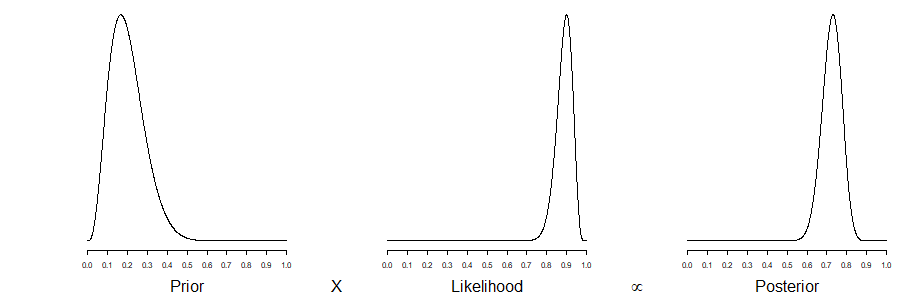
\includegraphics[width=6in]{fig2.png}
\end{center}
\caption{Prior, likelihood, and posterior for a nasty beta-binomial model \label{fig:bb_nasty}}
\end{figure}

The 95\% credible interval shows how mulish things have become. This interval (0.62 to 0.82) declares that the prior mean (0.2) is highly improbable. It also declares that the data mean (0.9) is highly improbable, so you're pretty much distrusting every aspect of this data analysis.

There's one more thing, though, that is very troubling about this analysis. Notice that the 95\% credible interval in this case has the same width as the interval reported earlier. You are haunted now by the equation that you thought you loved, prior sample size of 20 plus a data sample size of 60 equals a posterior sample size of 80. Your credible interval is too precise because it benefits undeservedly from the precision of a prior distribution that is clearly flawed. 

This is the sly dig in the Stephen Senn quote mentioned earlier. A vague expection plus a brief glimpse leads to a strong conclusion. When we humans see data that contradicts our expectation, our rational reaction is caution, but the Bayesian model plunges blindly ahead and assigns a posterior sample size of 80.

At this point, you want to crawl under a rock. Why oh why, you ask, did I use an informative prior. You want to take back your informative prior, but if you do, you're pretty sure that the Reverend Bayes will strike you down with a lightning bolt.

That's how I think you'd react, but maybe you're different. You might be thinking, now's not the time to get all wobbly. You didn't just pick that informative prior willy nilly. It was justified through a rigorous review of historical data or the careful elicitation of expert opinion. If you don't have the strength of will to stand by your informative prior, then you just aren't cut out to be a true Bayesian.

Whatever your perspective, wouldn't it be nice if you had something between the two extremes of a flat prior and an informative prior? Wouldn't it be nice to have a prior distribution that behaves like an informative prior when your data are consistent with the prior and behaves like a flat prior when your data are inconsistent with the prior?

\section{The hedging hyperprior}
\label{sec:hh}

The hedging hyperprior was originally proposed in \cite{jiang15} in the context of an informative gamma prior distribution on an exponential waiting time model. This paper will illustrate this same hyperprior in the setting of a beta-binomial model.

The hedging hyperprior adds a new hyperparameter, $\tau$, which (at least for now) is uniform on the interval 0 to 1. This choice is a bit too cautious, but it represents a good place to start the discussion.

Use this hyperparameter to modify the two parameters of the beta distribution. When $\tau$ is 1, the beta distribution remains unchanged from the classic beta-binomial formulation. When $\tau$ is zero, the beta distribution changes to a flat prior. For values of $\tau$ between 0 and 1, the beta distribution becomes a weaker, but still informative prior distribution.

The JAGS code (also shown in Table \ref{tab:hedging_code}) is only four lines longer than the code for a beta-binomial model. Note the inclusion of an extra line of code at the end to track the posterior sample size.

\linespread{1}

\begin{table}
\caption{The beta-binomial model with the hdeging hyperprior.\label{tab:hedging_code}}

Hedging hyperprior formulation \\
\\
$\tau \sim Uniform(0, 1)$\\
$\pi \sim beta(1+\tau(\alpha-1), 1+\tau(\beta-1))$\\
$x \sim Binomial(n, \pi)$\\
\\
JAGS code for the hedging hyperprior

\begin{verbatim}
  model {
    tau ~ dunif(0,1)
    a0 <- 1+tau*(a-1)
    b0 <- 1+tau*(b-1)
    pi ~ dbeta(a0,b0)
    x ~ dbin(p,n)
    post.n <- a0+b0+n
  }

\end{verbatim}
(R code remains the same)
\end{table}

\linespread{1.6}

How does the hedging hyperprior perform with data inconsistent with the prior? Quite well actually. Consider the previous example with 54 successes out of 60 trials, but modify the beta(4, 16) prior by adding the hedging hyperparameter. The mean estimate of $\pi$ is 0.88 (see Table \ref{tab:hedging_output_nasty}), which is very close to the proportion observed in the data. The mean estimate for $\tau$ (0.049) and for the posterior sample size (62.9, but note that a harmonic mean might be a better summary statistic) both indicate that the precision of your posterior is not unfairly enhanced by a flawed prior distribution.

\linespread{1}
\begin{table}
\caption{Output from the hedging model with nasty data.  \label{tab:hedging_output_nasty}}
\begin{verbatim}
##            Mean      SD Naive SE Time-series SE
## pi      0.87673 0.04147 0.001311       0.001311
## post.n 62.87591 0.79532 0.025150       0.052324
## tau     0.04866 0.04418 0.001397       0.002907
\end{verbatim}
\end{table}

Now consider the hedging hyperprior for the setting where the data are consistent with the prior (Table  \ref{tab:hedging_output_nice}). The posterior mean for binomial proportion is close to the mean of the data. The posterior mean of $\tau$ (0.53) and of the posterior sample size (71.5) both indicate a reduction in the weight placed on the prior distribution, but not as much of a reduction as when the data are inconsistent with the prior distribution. 

\linespread{1.6}


\linespread{1}

\begin{table}
\caption{Output from the hedging model with nice data.  \label{tab:hedging_output_nice}}
\begin{verbatim}
##           Mean      SD Naive SE Time-series SE
## pi      0.2883 0.05356 0.001694       0.001694
## post.n 71.4545 4.92925 0.155876       0.201223
## tau     0.5252 0.27385 0.008660       0.011179
\end{verbatim}
\end{table}

\linespread{1.6}

There's a simple graphical illustration that allows you to teach students how the hedging hyperior works. Adding a hyperparameter to the prior distribution produces a prior surface, as shown in Figure \ref{fig:hedging_surface}.

\begin{figure}
\begin{center}
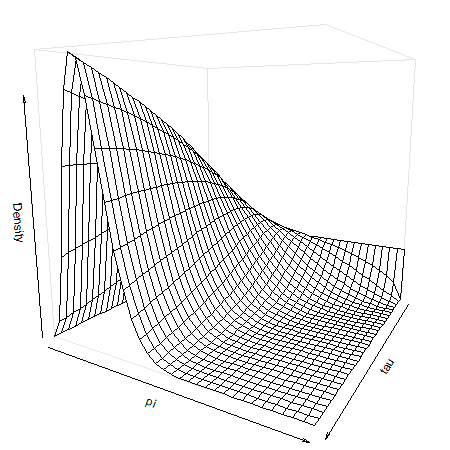
\includegraphics[width=3.25in]{fig3.png}
\end{center}
\caption{Prior surface for the hedging prior \label{fig:hedging_surface}}
\end{figure}

You should think about the shapes of this surface for fixed values of $\tau$ and for fixed values of $\pi$ by "slicing" the surface.

\begin{figure}
\begin{center}
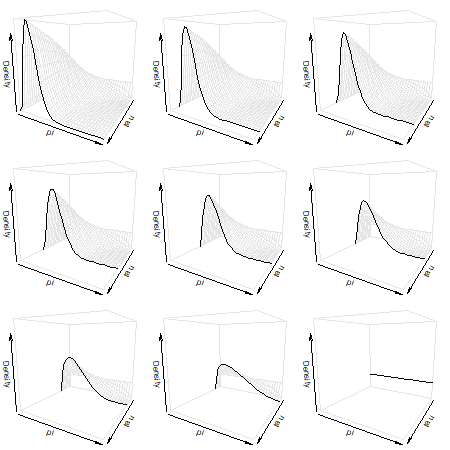
\includegraphics[width=3.25in]{fig4.png}
\end{center}
\caption{Prior surface with different values of $\tau$ highlighted \label{fig:hedging_surface1}}
\end{figure}

For a fixed value of $\tau$, the slices are easily recognized by your students as different beta distributions (Figure \ref{fig:hedging_surface1}). For $\tau$=1, it is the informative prior, beta(4,16). For smaller values of $\tau$, the beta distributions get spread out more, corresponding to a weaker prior. For very small values of $\tau$, the beta distribution converges on a uniform distribution.

\begin{figure}
\begin{center}
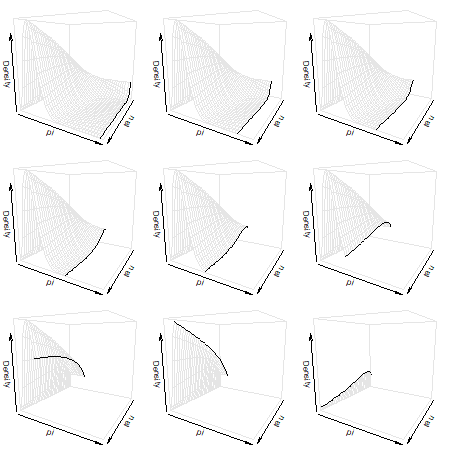
\includegraphics[width=3.25in]{fig5.png}
\end{center}
\caption{Prior surface with different values of $\pi$ highlighted \label{fig:hedging_surface2}}
\end{figure}

Now let\'s look at slices for fixed values of $\pi$ (Figure \ref{fig:hedging_surface2}). When $\pi$ is very large, your students will notice that the distribution of $\tau$ is skewed strongly towards zero. For moderate values of $\pi$, the skew reverses. For very small values of $\pi$, it reverts again to skew towards zero. This offers your students some intuition on why the hyperparameter downweights the prior sample size only for proportions that are discrepant from the informative prior.

\begin{figure}
\begin{center}
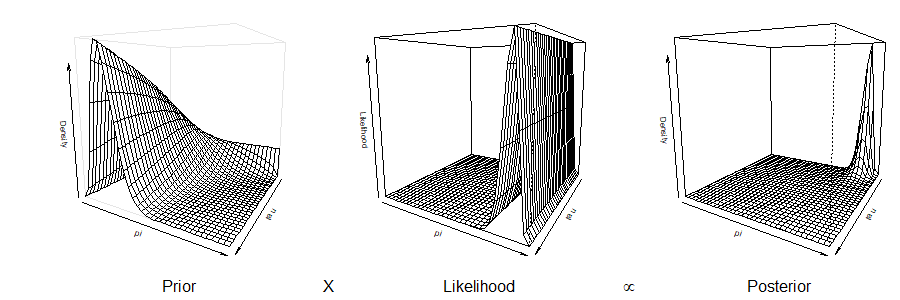
\includegraphics[width=6.25in]{fig6.png}
\end{center}
\caption{Posterior surface for data with 54 / 60 successes. \label{fig:hedging_surface3}}
\end{figure}

You can also visually show students how the likelihood surface works. The likelihood is unaffected by the hyperparameter $\tau$, and tends to enhance values of $\pi$ close to the mean of the data. Figure \ref{fig:hedging_surface3} shows the likelihood surface for the case where the data are inconsistent with the prior distribution (54 successes and 6 failures). You can see the likelihood acting like a steam roller that flattens out all the small and moderate values of $\tau$. What is left is a small peak in the upper left corner corresponding to small values of $\tau$ and large values of $\pi$.

\begin{figure}
\begin{center}
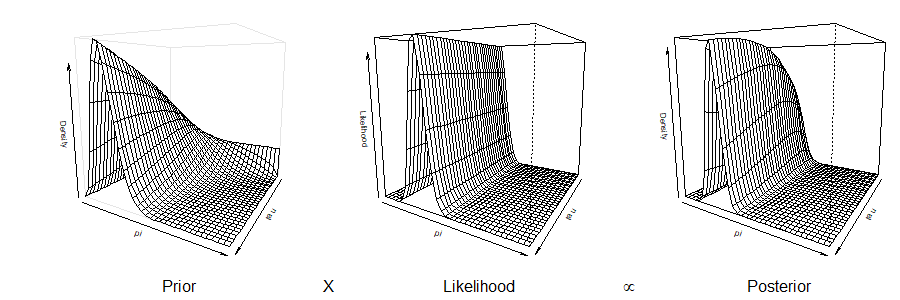
\includegraphics[width=6.25in]{fig7.png}
\end{center}
\caption{Posterior surface for data with 18 / 60 successes. \label{fig:hedging_surface4}}
\end{figure}

Figure \ref{fig:hedging_surface4} shows a setting where the data are consistent with the prior distribution (18 successes and 42 failures). Here you can show how the likelihood enhances the existing peak in the prior for moderate values of $\pi$. These are also where the value of $\tau$ is large, showing how it keeps greater weight on the prior distribution than the earlier discrepant case.

Since the likelihood gets narrower and narrower as the sample size increases, the slices of the prior surface for fixed values of $\pi$ become very important. They represent the limiting case for the hedging hyperprior. In particular, the expected value of $\tau$ for a fixed value of $\pi$ represents how much the informative prior will end up getting discounted in the limiting case. 

You can plot this mean versus $\pi$ to get the hedge trace, a simple two dimensional plot that shows you where serious discounting of the informative prior starts (Figure \ref{fig:hedge_trace}).

Notice that placing using a uniform distribution for the hyperprior leads to some amount of downweighting, even when the data and the prior agree perfectly. This is not too surprising, as the uniform distribution has a mean of 0.5. The hedge trace can help you evaluate the impact of alternative hyperprior distributions (as we will discuss in Section \ref{sec:pr}).

\begin{figure}
\begin{center}
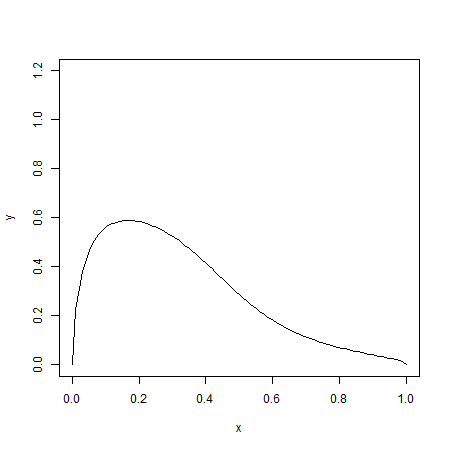
\includegraphics[width=3in]{fig8.png}
\end{center}
\caption{Hedge trace. \label{fig:hedge_trace}}
\end{figure}


\section{Equivalence to the Modified Power Prior}
\label{sec:equiv}

The Modified Power Prior has been proposed as a way to downweight a bad historical prior distribution. The approach is effective, but the mathematical notation is a bit daunting.

Consider the historic prior and the data as two sets of data, D0 and D. If, for example, your informative prior were  beta(4, 16), then you would create a pseudo data set with (4-1=3) successes and (16-1=15) failures. Apply this pseudo data to a flat prior ($\pi_0(\theta)$), get a posterior distribution the resembles your informative prior.

$\pi(\theta | D_0) \propto L(\theta|D_0)\pi_0(\theta)$ 

Then use $\pi(\theta | D_0)$ use that as your prior distribution for the new data.

$\pi(\theta | D,D_0) \propto L(\theta|D)\pi(\theta | D_0)$  

What \cite{ibrahim03} suggested is that you could downweight the historical prior by raising the historical likelihood to the power.

$\pi(\theta | D_0, \tau) \propto L(\theta|D_0)^{\tau}\pi_0(\theta)$

With $\tau$=1, you get the full strength of the historical prior and with $\tau$=0 you wipe out the historic data and are left with just a flat prior. This formulation requires a fudge factor ($\int L(\theta|D_0)^{\tau}\pi_0(\theta)d\theta$) to make things work nicely.

It is fairly easy to show that hedging hyperprior in the beta-binomial model is equivalent to the Modified Power Prior. Notice that

$L(\theta|D_0)^{\tau}=\left(\frac{(\alpha+\beta-2)!}{(\alpha-1)!(\beta-1)!}\theta^{\alpha-1}(1-\theta)^{\beta-1}\right)^\tau$

is proportional to

$\theta^{(\alpha-1)\tau}(1-\theta)^{(\beta-1)\tau}$

If you multiply this by a uniform prior for theta and apply the fudge factor, you get a $beta(1+(\alpha-1)\tau,1+(\beta-1)\tau)$ distribution for $L(\theta|D_0)$.

\section{Alternative hyperpriors}
\label{sec:pr}

The uniform(0,1) hyperprior is perhaps not the best choice for a hyperprior. It still significantly downweights the prior distribution even when the data are consistent with the prior. This should not be too surprising. The uniform(0,1) hyperprior has a mean of 0.5. The increasing peaks associated with stronger priors on $\pi$ will help somewhat but even with perfect agreement between the data and the prior, the hyperprior still reduces the strength of the prior to 60\% of the strength of the original prior.

\begin{figure}
\begin{center}
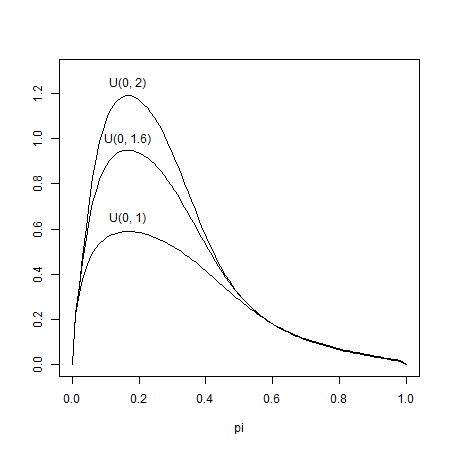
\includegraphics[width=3in]{fig9.png}
\end{center}
\caption{Hedge trace for different uniform distributions. \label{fig:hedge_trace}}
\end{figure}

A very simple way to improve the performance of the hedging hyperprior is to use a  uniform(0,2) hyperprior. The hedge trace for this hyperprior produces much less discounting of the prior when your data agrees with the prior. In fact, if the agreement is stronger than you'd normally expect, you get a small bonus.

If you dislike the idea of a bonus, a uniform(0, 1.6) distribution will guarantee that the posterior mean of $\tau$ never exceeds 1. This guarantee appears to hold across a broad range of prior distributions on $\pi$.

You are also not restricted to just a uniform distribution for the hedging hyperprior. A bit too extreme, perhaps, is the suggestion in \cite{Hobbs11} to use a beta(10,1) if you want to strongly encourage reliance on the informative prior and a beta(1,10) if you want to strongly discourage reliance on the informative prior. But skewing slightly to the left or right from a uniform distribution does allow you to fine tune the ranges where you want to strongly downweight the prior distribution.

You can also substitute a Bernoulli distribution for the uniform hyperprior. This effectively provides a weighted average between a posterior based on the full informative prior and a posterior based on a flat prior, with the relative weights controlled by the degree to which the data agrees/disagrees with the informative prior. This approach is equivalent to the robust meta-analytic prior proposed in \cite{schmidli14}. 

\section{Conclusion}\begin{figure}
\begin{center}
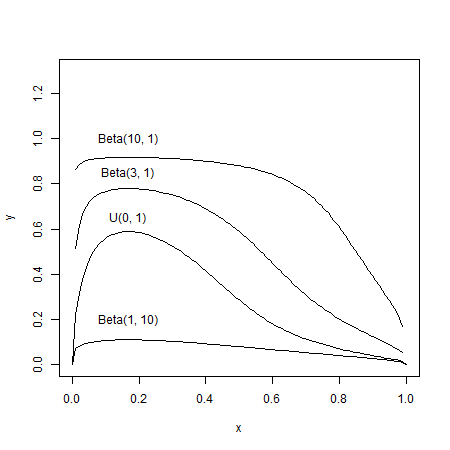
\includegraphics[width=3in]{fig10.png}
\end{center}
\caption{Hedge trace for different beta distributions. \label{fig:hedge_trace}}
\end{figure}

\label{sec:conc}

The hedging hyperprior is a simple modification that you can use whenever you have an informative prior distribution and the distribution can be reparameterized to include a measure of the prior sample size. It offers a simple visualization that helps students new to Bayesian statistics see how to borrow strength from an informative prior, but only to the extent to which the informative prior agrees with the data.

The hedge trace, a graph of how the mean of the hyperparameter changes as the main parameter varies, helps you show how much disagreement between the prior is needed before you see significant downweighting of the prior distribution.

For the beta-binomial case, the hedging hyperprior is equivalent to the Modified Power Prior. The advantage to formulating the problem as the hedging hyperprior is that it makes it easy to see how to use standard Bayesian software like BUGS, JAGS, or STAN. Also, the hedging hyperprior is easier to visualize, allowing you to readily discern its behavior in cases consistent with and discrepant from the informative prior.

The beta-binomial model is an ideal setting for understanding how the hedging hyperprior works because the parameter space is only two dimensional and is bounded in all directions. Further research is needed to explore the role of the hedging hyperparameter in more complex models and to better understand the performance of various alternative hyperprior distributions.

\section{Bibliography}

\bibliographystyle{Chicago}

\bibliography{hedging}
\end{document}
